\documentclass[10pt,twocolumn,letterpaper]{article}

\usepackage{icb}
\usepackage{times}
\usepackage{epsfig}
\usepackage{graphicx}
\usepackage{amsmath}
\usepackage{amssymb}
\usepackage{listings}

% Include other packages here, before hyperref.

% If you comment hyperref and then uncomment it, you should delete
% egpaper.aux before re-running latex.  (Or just hit 'q' on the first latex
% run, let it finish, and you should be clear).
%\usepackage[pagebackref=true,breaklinks=true,letterpaper=true,colorlinks,bookmarks=false]{hyperref}

\icbfinalcopy % *** Uncomment this line for the final submission

\def\icbPaperID{****} % *** Enter the IJCB Paper ID here
\def\httilde{\mbox{\tt\raisebox{-.5ex}{\symbol{126}}}}

% Pages are numbered in submission mode, and unnumbered in camera-ready
\ificbfinal\pagestyle{empty}\fi
\begin{document}

%%%%%%%%% TITLE
\title{\LaTeX\ Author Guidelines for ICB 2015 Proceedings [Based on CVPR]}

\author{Thomas Bergmueller\\
Authentic Vision, University of Salzburg\\
Salzburg, Austria\\
{\tt\small tb@authenticvision.com}
% For a paper whose authors are all at the same institution,
% omit the following lines up until the closing ``}''.
% Additional authors and addresses can be added with ``\and'',
% just like the second author.
% To save space, use either the email address or home page, not both
\and
Eleftherios Christopoulos, Martin Schnoell\\
University of Salzburg\\
Salzburg, Austria\\
{\tt\small \{mschnoell, echristopoulos\}.aise-m2013@fh-salzburg.ac.at}
}

\maketitle
\thispagestyle{empty}

%%%%%%%%% ABSTRACT
\begin{abstract}
   The ABSTRACT is to be in fully-justified italicized text, at the top
   of the left-hand column, below the author and affiliation
   information. Use the word ``Abstract'' as the title, in 12-point
   Times, boldface type, centered relative to the column, initially
   capitalized. The abstract is to be in 10-point, single-spaced type.
   Leave two blank lines after the Abstract, then begin the main text.
   Look at previous ICB abstracts to get a feel for style and length.
\end{abstract}

%%%%%%%%% BODY TEXT
\section{Introduction}
TODO

\section{Data set}
\label{sec:data}
For testing, we employ the MIT indoor scene recognition database \cite{indoorScenes}. The authors in \cite{indoorScenes} already point out desireable results by comparing the performance of 
\begin{itemize}
	\item Visual words with SIFT-Features
	\item Gist features \cite{oliva06}, which is a content-based method and
	\item RGB-classification \cite{indoorScenes}, where mean RGB-images of the particular scenes were used for training.
\end{itemize}

Along the database, the authors ship two text files, one, \emph{TrainImages.txt}, listing the pre-selected training data and another one, \emph{TestImages.txt}, listing the pre-selected test data. We stick to this pre-defined splitting of the data set since this ensures comparability with results found in literature. The data set contains a total of 15620 images showing 67 indoor scene categories. The data is structured in folders, where each folder represents one scene category. Interestingly, although the authors claim in \cite{indoorScenes} that the data set using these pre-selection files is partitioned resulting in 80 training images and 20 per class, we observe that although the total number of files ($67*(20+80) = 6700$) is correct, some classes in training and testing have an unexpected number of files, e.g. 79 for training or 23 for testing. Despite that, we stick to the proposed selection for the sake of comparable results.

The structure of the data base allows to retrieve the ground truth, namely the category each image belongs to from the full path to a particular image. We employ an image processing pipeline, where we store results after each intermediate steps in a separate folder. Doing so, we take advantage of firstly being forced to create a sensible interface between the detection stages and secondly, we cut down on computation time in the development process when parts of just one step in the pipeline is changed. However, we change the labeling of the $C=67$ classes from alphanumeric to integer labeling to simplify processing with Matlab. Additionally, \cite{indoorScenes} suggests grouping into five large groups, Store, Home, Public spaces, leisure and Working place. We keep this as an option by training the SVM differently if need be, namely by mapping the class labels to the five categories.



\section{Processing pipeline}
In order to classify scenes, we use the processing pipeline shown in figure \ref{fig:pipeline}. We propose the following structure to store data for exchange between the different steps of the pipeline:


\begin{lstlisting}
{
	x,
	targets,
	class
}
\end{lstlisting}

The x-field of the structure corresponds to the actual content of a data set. This could be RGB-values, Greyscale values, high- and low-level feature vectors or empty.

\begin{figure}
	\begin{center}
		

	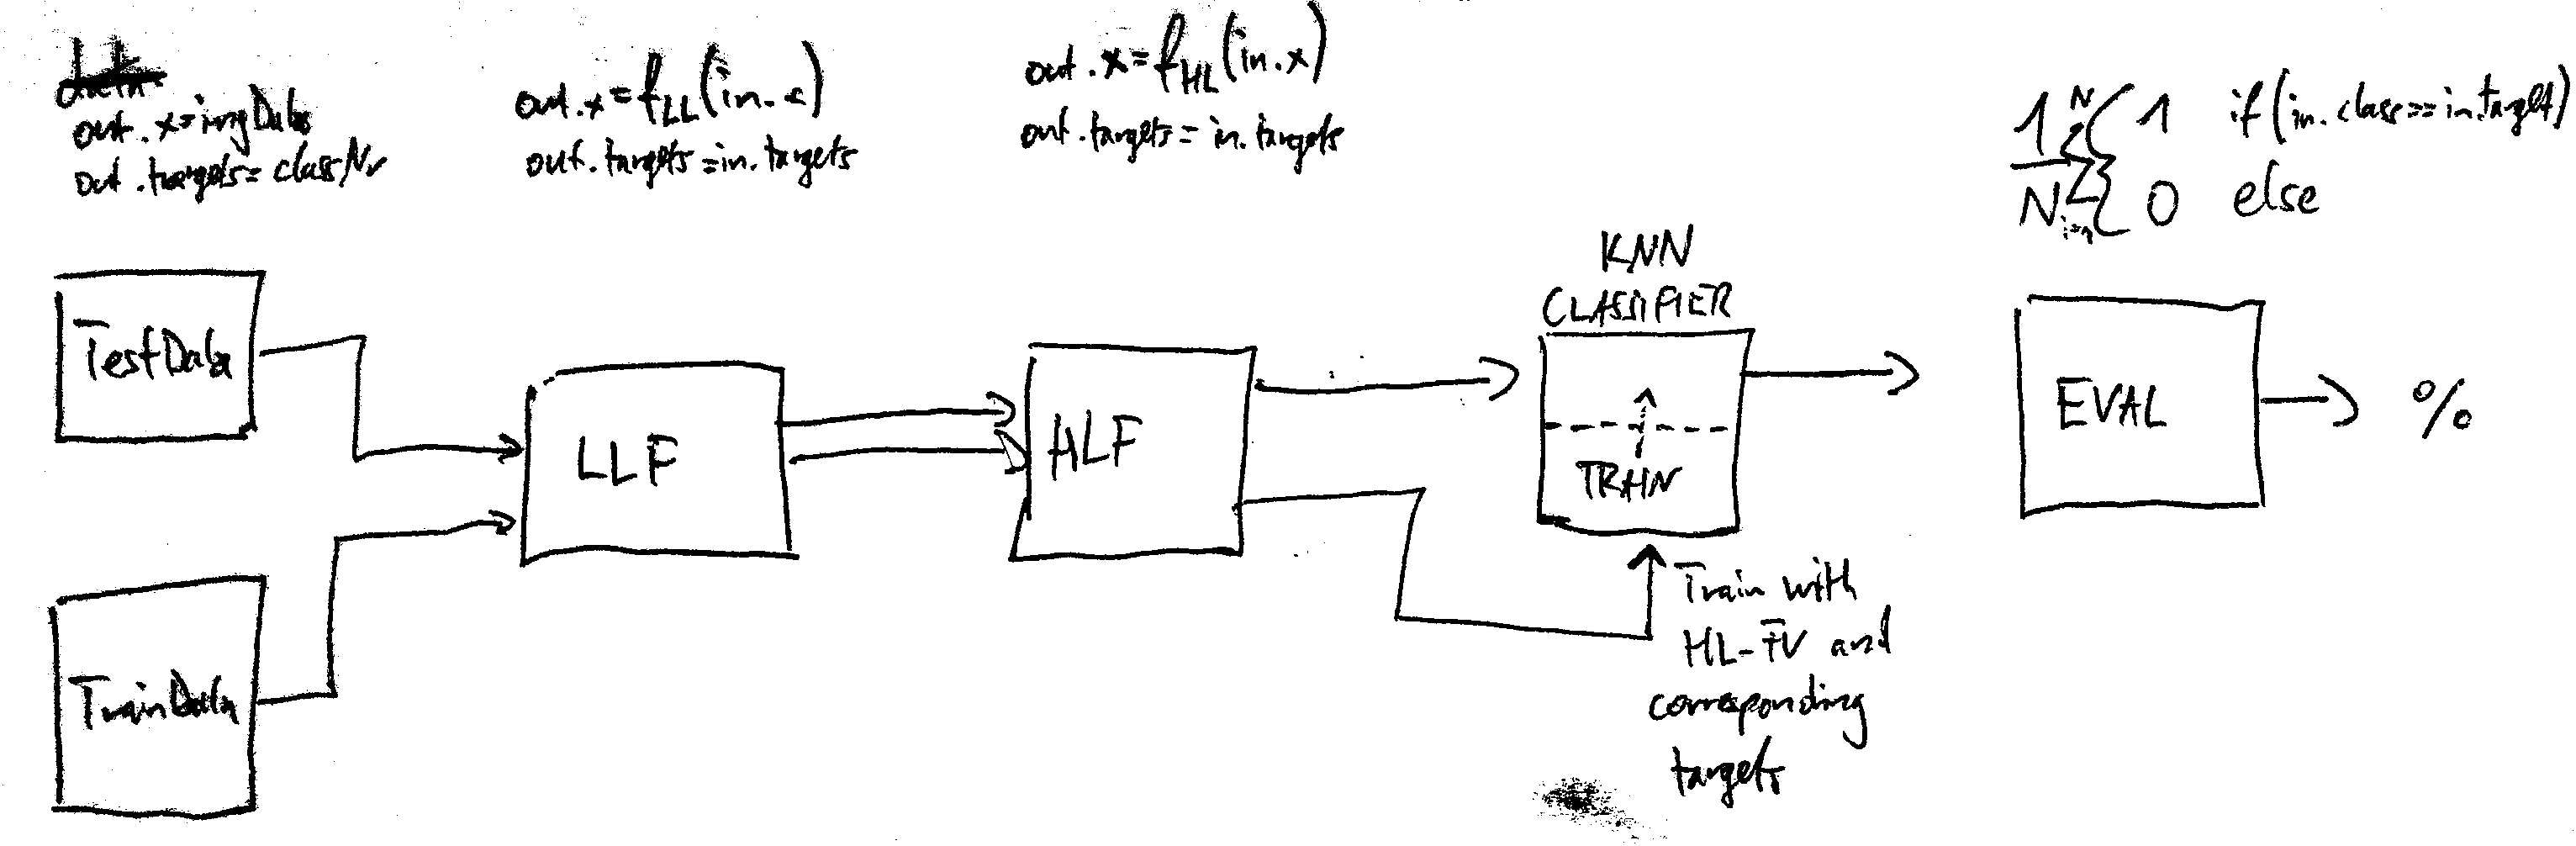
\includegraphics[width=\textwidth]{img/pipeline}
	\label{fig:pipeline}
	\caption{Processing pipeline of test- and training-data}
		\end{center}
\end{figure}

\subsection{Classifier}
For classification, we use (as also in \cite{indoorScenes}) a support vector machine (SVM). The SVM is trained using the high-level features of the training data together with the class labelling retrieved from the file names, i.e. the folder name they are stored in, of the stored high-level features.




{\small
\bibliographystyle{ieee}
\bibliography{egbib}
}

\end{document}
